\chapter{Background}\label{cha:theory}
This chapter includes relevant background information about the main topics of this report. The purpose of the chapter is to give the reader some basic knowledge and understanding about the touched topics to facilitate further reading of the report.
\section{Computer graphics}\label{computergraphics}
Distance fields and text renderering are subjects closely related to computer graphics. Therefore it is important to understand some basic concepts about computer graphics when reading this report. Two important concept in the context of this thesis are polygons and textures. A polygon is a figure bound together by a finite chain of straight line segments. The corners of the polygon are called vertices and are defined as coordinates in space. A usual representation of a polygon is a list of vertices where the vertices are ordered in a way that every vertice is connected to the next vertice in the list by a line segment. A texture is a representation of an image. The texture is usually represented as a one or two dimensional array with a 8 or 32 bit value per pixel. 

When drawing an image or texture to the screen it has to be mapped to a polygon first. When working in two dimensions an useful polygon for mapping textures to is the quad which is the polygon with four corners. The process of drawing a texture to a quad on the screen follows. The quad is created by creating a list of vertices. A list of texture coordinates is created. Texture coordinates defines which part of the texture should be drawn on the quad. The texture is uploaded to the GPU together with the list of vertices and the list of texture coordinates. Shaders written by the programmer runs and the texture is drawn on the quad. There are two shaders of importance within the scope of this thesis, the vertex shader and the fragment shader. The vertex shader is run one time for every vertex. In the case with a texture mapped to the quad the vertex shader would just pass through the input values. The next shader run is the fragment shader. The fragment shader is run once for every candidate pixel on the screen. The output data from the vertex shader is interpolated before sent as input to the fragment shader. The interpolation is needed because it is very rare that every vertice maps exactly to one pixel on the screen. The interpolation is done for every variable that is sent to the fragment shader. An schoolbook example of the interpolation is the colored triangle. The three vertices of the triangle get three different colors sent to the corresponding vertex shader. The vertex shader pass through the colors and the GPU interpolates the colors to a separate color for each pixel. This will create a color gradient between the three corners where each pixel has a unique color. 
\begin{figure}[H]
\centerline{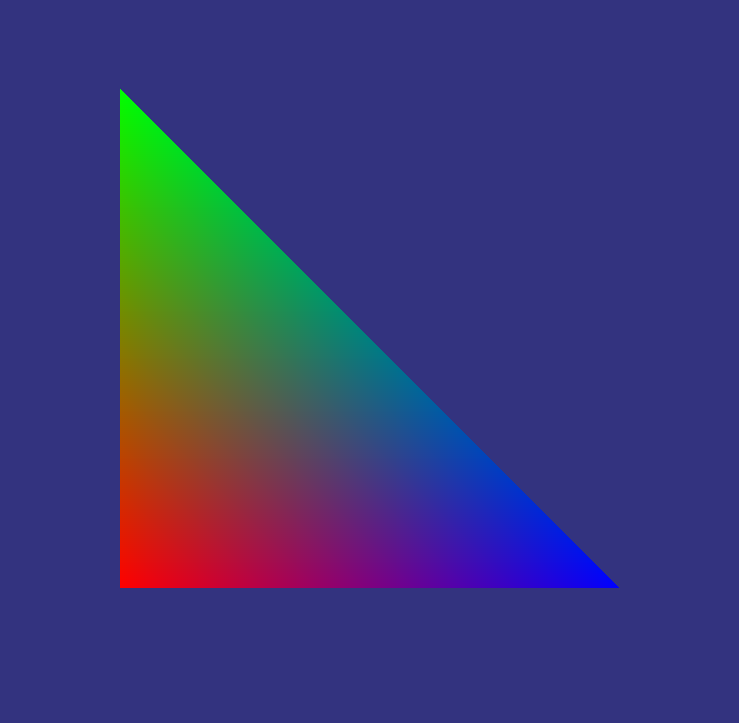
\includegraphics[scale=0.35]{triangleInterpolation}}
\caption{An example of the interpolation between the vertex and fragment shader on the GPU}
\end{figure}
\section{Basic text rendering}\label{textrendering}
Text rendering is a non trivial subject in computer graphics and has been for a long time. There are many different ways to render text to a screen. A common way is to pre render all the glyphs of a font to an image. The part of the texture corresponding to a specific glyph can then be mapped as a texture to a quad and rendered on the screen. Another way is to use some library to render the text to an image and use it to texture a quad \citep{FreeType}. Both of the above mentioned methods have some drawback, for example the text can not be scaled up without losing the smooth edges and the images takes a lot of memory if you want to have high resolution on the text.

When rendering a text it is really important that every glyph is positioned relative other glyphs as specified in the font file. Every glyph in a font has visual information stored in the font file. For example the OpenType and the TrueType\texttrademark{} font format have information about advance, kerning, height, widht etc\citep{OpenType, TrueType}.

Without kerning it might be hard to get a good looking text if the font is not built in a way that kerning is not a factor. Kerning is displacement along the axis of the advancing direction of the text. A kerning value can be positive or negative and is a function of two parameters, the previous letter and the current letter. A negative kerning value is the most common and it means that the current glyph will be moved backwards relative to the advancing direction of the text and a positive value means that it will be moved forward. To get a better understanding of what kerning is take the strings ``AV'' and ``AA'' as an example. It is obvious that the left part of ``V'' is hanging above the ``A'' but that is not the case in the second string where ``A'' is followed by an ``A''. This is because the kerning table in the font has a negative entry for the combination ``AV'' but not for the combimation ``AA''. \citep{FreeTypeKern}

\begin{figure}[H]
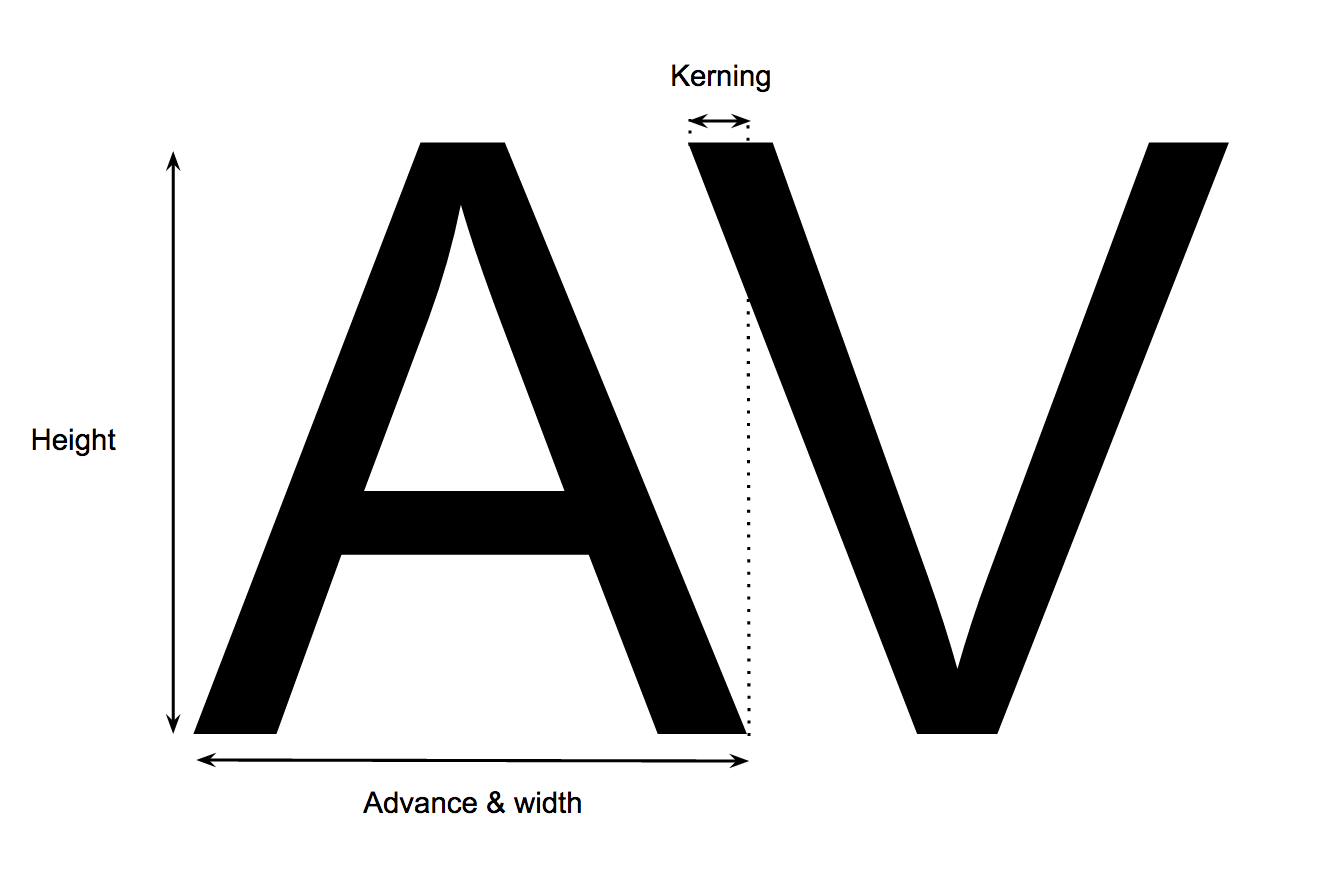
\includegraphics[scale=0.25]{glyph_kerning}
\caption{Illustration of how kerning works}
\end{figure}

Another important concepts when rendering text is the baseline. A text can be placed on different baselines located on different heights. The baselines used in this thesis work is top, hanging, middle, alphabetic, ideographic and bottom. The most commonly used baseline is the alphabetic baseline which is used for example when writing english text on a piece of paper.

\begin{figure}[H]
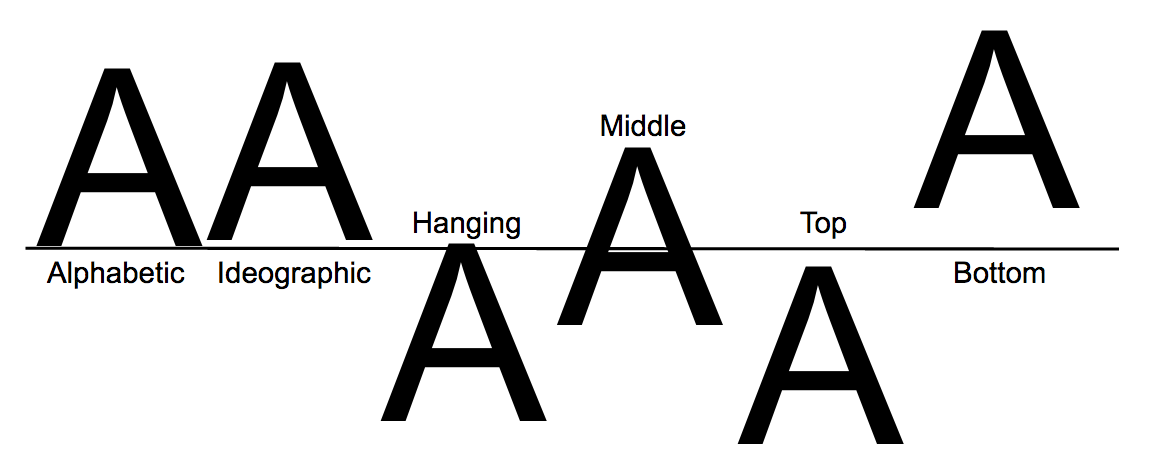
\includegraphics[scale=0.25]{glyph_baseline}
\caption{Some baselines}
\end{figure}

\section{Distance fields}\label{distancefield}
Binary images are frequently used in image processing \citep{Ragnemalm:1993}. A binary image is an image with only one binary value per pixel. This will limit the image to only contain two values or colors. One example of an image that could be represented as a binary image is a picture of a white letter on a black background. In this case white would be represented as 0 and black as 1 or vice versa.

A distance transform is the transform of an input binary image to an output image called distance field or distance map \citep{rosenfeld1966}. The values of the distance field pixels represents the closest distance by some distance metric to an arbitrary shape in the input image. The distance metric can differ between different applications but the most commonly used distance metric is the euclidean distance metric which is also called real distance. If euclidean distance metric is used when doing the distance transform it is called euclidean distance transform(EDT). Other distance metrics that can be used in distance transforms are the city-block distance metric and the chessboard distance metric. When using city-block distances it is only allowed to travel horizontally or vertically in a grid with the cost of one. Chessboard distance metric is an extension of city-block distance metric where it is also allowed to travel diagonally with the cost of one. 

A distance field can be signed or unsigned. An unsigned distance field only maps the distances either inside the shape or outside the shape while a signed distance field maps the pixels inside the shape with negative distances and the outside of the shape with positive distances or vice versa.

Distance fields have many good advantages compared to other methods for storing shapes like boundary representation. One of the most obvious advantages are that a distance field represents more than just the boundary. For example a signed distance field also represents the environment around the boundary, both the interior and the exterior. This makes it easy to check if a point is inside or outside a shape by checking the value of that point in the distance field. It is also easy to move the boundary of the object by just changing the threshold value determining where the boundary is located. \citep{Jones2006}

\section{Beziér curves}\label{bezier}
A beziér curve is defined in space or the plane as two endpoints and a number of control points which are blended together with one blending function per point. The number of control points depends on the degree of the beziér curve. The most commonly used beziér curves are the cubic beziérs with four points and the quadratic beziérs with three points. The quadratic and the cubic beziér are defined as follows.\vspace{\baselineskip}\newline
\begin{math}
B(t) = (1-t)^2P_0+2t(1-t)P_1+t^2P_2, t\in[0, 1] 
\end{math} \vspace{\baselineskip}\newline
\begin{math}
B(t) = (1 - t)^3P_0 + 3t(1 - t)^2P_1 + 3t^2(1 - t)P_2 + t^3P_3, t\in[0, 1]
\end{math} \vspace{\baselineskip}\newline
The quadratic beziér has $P_0$ and $P_2$ as endpoints and $P_1$ as a control point. The cubic beziér has $P_0$ and $P_3$ as endpoints and $P_1$ and $P_2$ as control points. The sum of the blending functions for both quadratic beziérs and cubic beziérs is always equal to 1 for any t in the function domain.\citep{PFNP}

\begin{figure}[H]
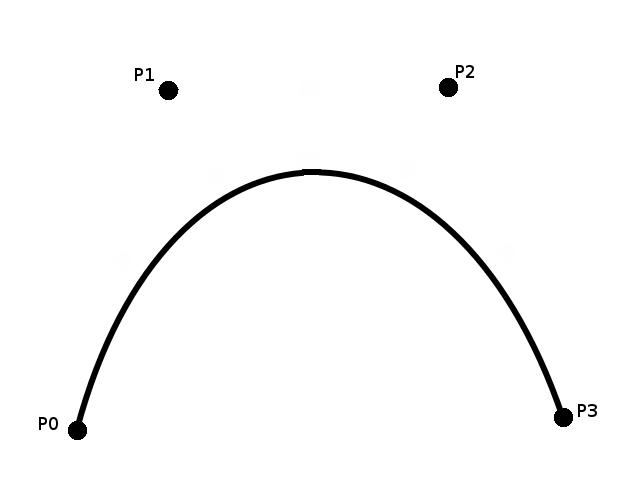
\includegraphics[scale=0.5]{bezier}
\caption{A cubic beziér curve}
\end{figure}

One beziér curve can not represent arbitrary curves, therefore it is important to be able to connect several beziérs to a path to be able to describe more complex shapes. When connecting curves, continuity between the curves is an important concept to consider. Parametric continuity is a measure that will have importance of the appearance of the curve. There are three levels of parametric continuity.\vspace{\baselineskip}\newline
\begin{math}C^0\end{math} = The curves meet\newline
\begin{math}C^1\end{math} = The derivative for the both curves are equal where the curves meet\newline
\begin{math}C^2\end{math} = The second derivative for the both curves are equal where the curves meet\vspace{\baselineskip} \newline
Another measure that can be used for continuity is geometric continuity which is almost the same as parametric continuity. The only difference is that geometric continuity only require the derivatives of $G^1$ and $G^2$ to be proportional and not equal. Given two cubic beziér curves p defined by $p_1$, $p_2$, $p_3$ and $p_4$ and q defined by $q_1$, $q_2$, $q_3$ and $q_4$. Assume that p and q are placed in a way that $p_4=q_1$. This will trivially fulfill the requirement for $C^0$ because they share one endpoint and $p(1)=q(0)$. $C^1$ continuity, $p'(1)=q'(0)$ will be fulfilled if $p_3$, $p_4$ and $q_1$ are located on the same line. C2 continuity $p''(1)=q''(0)$ will be fulfilled if  $p_3$, $p_4$ and $q_1$ are located on the same line and $|p_4 - p_3| = |q_2 - q_1|$ which means that the distance from $p_3$ to $p_4$ must be equal to the distance from $p_4$ to $q_2$.\citep{PFNP}

An example of an application of beziérs are fonts. Every glyph in a font are stored as a number of straight lines and beziér curves, either cubic or quadratic.\citep{phinney2001} Even though beziérs are used in fonts it is not a trivial problem to draw a beziér to the screen. Beziér curves are hard to draw because the lowest level graphics hardware can only draw polygons and line segments. This is solved by approximating smooth curves to line segments before drawing\citep{shreiner2009opengl}. Another problem with beziér curves is that it is time consuming to find the closest point on a beziér curve from an arbitrary point. To solve this problem $(p-q(t))q'(t)=0,$ where $t\in[0, 1] $, p is a point in space and q is a beziér curve, has to be solved\citep{xiaodiao}. This implies that a quintic polynomial needs to be solved to find the closest point on a cubic beziér curve given a point in space. 

De Casteljau’s algorithm can be used to subdivide a beziér curve recursively by using the properties of beziér curves to calculate new beziér points for both the left and the right part of the old beziér.\citep{fischer2000} A special case of the algorithm is to divide the curve at \begin{math}t=0.5\end{math} which gives a first curve \begin{math}t\in[0, 0.5]\end{math} and a second curve \begin{math}t\in[0.5, 1]\end{math}. An example of this subdivision for a cubic beziér is presented in figure \ref{fig:decasteljaus} below. The first curve is described by the points \begin{math}p_0\end{math}, \begin{math}p_{01}\end{math}, \begin{math}p_{012}\end{math} and \begin{math}p_{0123}\end{math} and the second curve is described by \begin{math}p_{0123}\end{math}, \begin{math}p_{123}\end{math}, \begin{math}p_{23}\end{math} and \begin{math}p_{3}\end{math}. The points for the new curves are derived from the initial curve described by \begin{math}p_{0}\end{math}, \begin{math}p_{1}\end{math}, \begin{math}p_{2}\end{math} and \begin{math}p_{3}\end{math}. The following calculations shows how the new beziér points are computed.\vspace{\baselineskip}\newline
\begin{math}
	P_{01}=\frac{P_0+P_1}{2}\newline
	P_{23}=\frac{P_2+P_3}{2}\newline
	P_{12}=\frac{P_1+P_2}{2}\newline
	P_{012}=\frac{P_{01}+P_{12}}{2}\newline
	P_{123}=\frac{P_{12}+P_{23}}{2}\newline
	P_{0123}=\frac{P_{012}+P_{123}}{2}
\end{math}\vspace{\baselineskip}\newline

\begin{figure}[H]
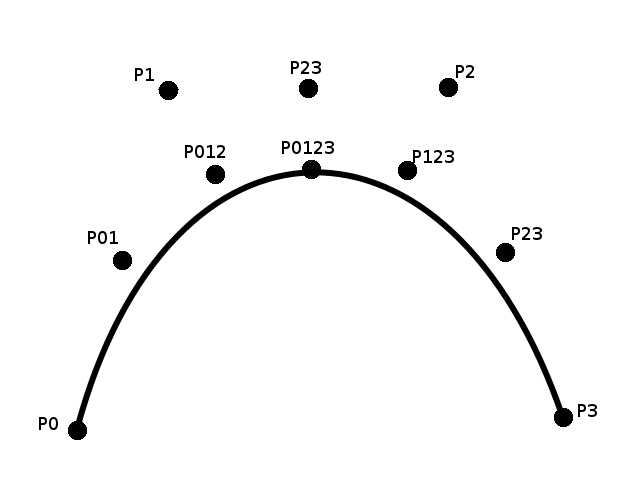
\includegraphics[scale=0.5]{de_casteljaus}
\caption{An illustration of the casteljau's algorithm splitting a cubic beziér at $t=0.5$}
\label{fig:decasteljaus}
\end{figure}

\section{Polygon filling}
Computer graphics is partly about drawing polygons to the screen but this does not make it a trivial problem. There are several algorithms for drawing a polygon to the screen where each one of them have their advantages and drawbacks. One algorithm that is used alot for this purpose is the scan-line polygon fill algorithm. The algorithm contains two main components. The first component is a sorted edge table which is an array of linked lists where each linked list corresponds to a row in the image. The second component is an active edge list which is an initially empty linked list of edge references. The x value for the lowest y value of each line segment is inserted into the edge table. The next step in the algorithm is to iterate through the edge table row by row. All edges in the active edge list that ended on the previous line are removed. All remaining values of the active edge list are updated to the intersection between the line segment and the current row. All values of the current row in the edge table are then inserted into the active edge list and the active edge list is then sorted by x value. The image can now be filled for the current row by using some fill rule. The odd even fill rule is easy to use by just iterating through the active edge list and filling the pixels between every pair of edges starting with an odd edge.

\begin{figure}[H]
\minipage{0.5\textwidth}
  
\includegraphics[width=\linewidth]{polygon}
  \caption{A case managed by odd even fill}\label{fig:awesome_image1}
\endminipage\hfill
\minipage{0.5\textwidth}
  
\includegraphics[width=\linewidth]{oddevenfillfail}
  \caption{A case not managed by odd even fill}\label{fig:awesome_image2}
	\label{fig:poly}
\endminipage\hfill
\end{figure}

The odd even fill rule only work if edges can not cross eachother. If edges cross eachother there might be filled where it should not be filled and vice versa. An example of this can be seen in figure \ref{fig:poly} where the odd even fill rule fails to fill the area in the middle. To handle this another fill rule has to be used, for example the non-zero winding number rule. This rule handle case of edges crossing eachother because the rule also takes into account in which direction the edges of the polygon are moving and increments a variable with different sign depending on that direction when crossing an edge.
\chapter{Related work}\label{cha:relatedwork}
\section{Early EDT algorithms}\label{earlyedt}
In a very often mentioned article \citet{Danielsson} proposed an improved way to generate distance maps by representing the output of the distance transform as a vector, separating the distance of the different dimensions. Danielsson also proposed two sequential algorithms 4SED (4-point Sequential Euclidean Distance mapping) and 8SED (8-point Sequential Euclidean Distance mapping) for calculating the EDT using his representation of distance. Both the 4SED algorithm and the 8SED algorithm consists of two consecutive picture scans where they incrementally update pixel values depending on nearby pixels. The 8SED algorithm is described in the following pseudocode.\vspace{\baselineskip}\newline
\begin{algorithm}[H]
\caption{First scan of the 8SED algorithm}
\begin{algorithmic}
\For{$j = 1 to N-1 step 1$}
	\For{$i = 0 to M-1 step 1$}
		\State L(i, j) = min(L(i, j), L(i-1, j-1)+(1, 1), L(i, j-1)+(0+1), L(i+1, j-1)+(1,1))\;
	\EndFor
	\For{$i = 1 to M-1 step 1$}
		\State L(i, j) = min(L(i, j), L(i-1, j)+(1, 0))\;
	\EndFor
	\For{$i = M-2 to 0 step 1$}
		\State L(i, j) = min(L(i, j), L(i+1, j)+(1, 0))\;
	\EndFor
\EndFor
\end{algorithmic}
\end{algorithm}
\vspace{\baselineskip}
\begin{algorithm}
\caption{Second scan of the 8SED algorithm}
\begin{algorithmic}[H]
%\KwData{M: Width, N: Height, L: Binary image of size MxN}
%\KwResult{L: Distance field}
%initialization\;
\For{$j = N-2$ to $0$ step $1$}
	\For{$i = 0$ to $M-1$ step $1$}
		\State L(i, j) = min(L(i, j), L(i-1, j+1)+(1, 1), L(i, j+1)+(0, 1), L(i+1, j+1)+(1, 1))\;
	\EndFor
	\For{$i = 1$ to $M-1$ step $1$}
		\State L(i, j) = min(L(i, j), L(i-1, j)+(1, 0))\;
	\EndFor
	\For{$i = M-2$ to $0$ step $1$}
		\State L(i, j) = min(L(i, j), L(i+1, j)+(1, 0))\;
	\EndFor
\EndFor
\end{algorithmic}
\end{algorithm}\vspace{\baselineskip}

The two scans are very similar. The only difference is that the first scan is done top down evaluating the pixels below and on the sides of the current pixel and the second scan is done bottom up evaluating the pixels above and on the sides of the current pixel\citep{Ragnemalm:1993}. The 4SED algorithm and the 8SED algorithm are not error free as \citet{Danielsson} proves in his article but he also claims that the errors are rare and small and are negligible for practical purposes. In 8SED and 4SED every pixel are visited a constant number of times. This makes the time complexity of 8SED and 4SED trivially $\mathcal{O}(mn)$, if m and n are the width respectively the height of the input image.
\section{Exact EDT algorithms}\label{exactEDT}
Distance transforms has been used in different applications in many years. The article from \citet{Danielsson} was not the first on the subject but the fact that the algorithms he proposed in his article are some of the most widely used\citep{edtcompare} makes it easy to call Danielsson one of the pionjeers on the subject. As mentioned earlier in this report, 8SED and 4SED are not exact. Exact algorithms for EDT has only been around since about the 1990s. In an article \citet{edtcompare} compares the execution time of exact EDT algorithms. The six algorithms compared in the test are \citet{meijster}, \citet{maurer}, \citet{eggers}, \citet{lotufo}, \citet{cuisenaire} and \citet{saito}. The conclusion of the comparison is that the algorithms from Meijster and Maurer are the fastest but Meijster's algorithm is preferred due to slightly better performance and the fact that it is easier to implement than Maurer's algorithm.

Meijster's algorithm consist of two separate phases. The first phase iterates through each column performing a distance propagation in both directions. This will create a new image \begin{math}g(i, j)\end{math} which is used in the second phase. The second phase iterates through each row left to right and right to left applying a function \begin{math}DT(x, y)\end{math} to calculate the output value of each pixel. The function depends on what distance metric is used. The function used for euclidean distance transform follows.\vspace{\baselineskip}\newline
\begin{math}
	DT(x, y) = \min\limits_{0\dots m}((x-i)^2+g(i)^2)
\end{math}\vspace{\baselineskip}\newline
With the same motivation for 4SED and 8SED the time complexity of Meijster's algorithm is $\mathcal{O}(nm)$, if m and n are the width respectively the height of the image.

\section{Improved distance measure for EDT algorithms}\label{limitEDT}
Calculating a distance transform of large size images can be very time consuming. There is a significant difference in computation time between creating a distance map from a 4096x4096 image and creating a distance map from a 64x64 image. For example, the 8SED and the 4SED algorithms both have time complexity O(n) where n is the number of pixels. Time complexity O(n) means that every pixel is visited a constant number of times when transforming the image. Assuming every pixel is visited once and one calculation is done per visit the larger image would require 4096 times more calculations than the smaller image. In an article from \citet{Green:2007}, distance fields are generated by using a 4096x4096 binary image of a glyph as input to a distance transform. The output from the distance transform is then downsampled to a 64x64 texture. Generating a distance field using a large input image makes the discrete set of possible boundary pixels more dense compared to if a smaller input image was used. The increased density of the possible pixel set helps decrease the calculation error of the distance field assuming subpixel distance measures is not used.

In an article, \citet{Gustavson:2011} shows that the calculation errors of distance transforms can be decreased by using information about the subpixel boundary between the foreground and the background pixels. In the article they use an anti-aliased greyscale input image to be able to locate the boundary in the pixels to get more precise distance measures between the pixel and the boundary. 

 They show that they get approximately the same amount of errors using their method on a 16x16 times smaller input image than by using the method Chris Green proposed in his article. The smaller input image increases the the execution time and decreases the memory consumption by a factor of approximately 30 times according to Gustavson and Strand.
